\documentclass[aspectratio=169,10pt]{beamer}

\usetheme{Madrid}
\usecolortheme{whale}

\usepackage{amsmath,amssymb}
\usepackage{booktabs}
\usepackage{graphicx}
\graphicspath{{./}{../../}}

\title[DupHunter: Scalable Duplicate Detection]{DupHunter: Scalable Duplicate Question Detection at Scale}
\subtitle{Mining 2.2 Million Stack Overflow Questions with Custom MinHash \& LSH on Spark}
\author[ENSF 612 Team]{
  Satyam Bhanot (WS1) \and
  Iesrat Jahan (WS2) \and
  Navjot Singh Shienh (WS3) \and
  Md Jubayer Khan (WS4)
}
\institute[UCalgary]{ENSF 612: Big Data Analytics --- Final Presentation}
\date{November 23, 2026}

\begin{document}

\begin{frame}
  \titlepage
\end{frame}

% -----------------------------------------------------------------------------
% Presenter: Satyam Bhanot (WS1)
% -----------------------------------------------------------------------------

\begin{frame}{1. Problem Formulation: Duplicate Questions on Stack Overflow}
  \begin{itemize}
    \item \textbf{Context:} Stack Overflow has 24,133,975 questions in this data release, and people keep asking the same thing in different words.
    \item \textbf{Why It Matters:} Community fragmentation, redundant expert effort, delayed answers for developers.
    \item \textbf{The Computational Bottleneck:}
      \begin{itemize}
        \item Pairwise comparison across $N = 2{,}204{,}200$ python questions requires:
          \[ \frac{N(N-1)}{2} \approx 2.43 \times 10^{12} \text{ comparisons (quadratic explosion)} \]
        \item At 10,000 comparisons/sec, exhaustive search needs about \textbf{7.7 years of compute}.
      \end{itemize}
    \item \textbf{Project Objective:} Build a sub-quadratic, distributed candidate generation pipeline on Apache Spark that gives up some recall to avoid comparing almost all pairs.
  \end{itemize}
  \vfill
  \footnotesize{\textit{Figure source: Question counts (\texttt{results/dataset\_stats.md})}}
\end{frame}

\begin{frame}{2. Big Data Characteristics \& Streaming ETL}
  \begin{itemize}
    \item \textbf{Dataset (Stack Exchange Archive):} 68.9 GB compressed XML archive; 2.2M Python questions; 517k Super User questions.
    \item \textbf{Big Data 5 Vs Addressed:}
      \begin{itemize}
        \item \textbf{Volume:} Scaled from single-laptop local mode to a multi-node cluster.
        \item \textbf{Variety:} Unstructured text, semi-structured HTML (\texttt{<code>}, \texttt{<pre>}), and relational duplicate graphs.
        \item \textbf{Velocity \& Skew:} Time-series question arrivals with heavy popularity skew on common tags.
      \end{itemize}
    \item \textbf{Streaming ETL Pipeline (Contract C1):}
      \begin{itemize}
        \item Streaming XML decompression (\texttt{7z x -so}) directly into year-partitioned Parquet tables without unpacking to disk.
        \item Output tables: \texttt{posts\_meta}, \texttt{posts\_text}, \texttt{post\_links}.
      \end{itemize}
  \end{itemize}
  \vfill
  \footnotesize{\textit{Figure source: Dataset statistics (\texttt{results/dataset\_stats.md})}}
\end{frame}

\begin{frame}[shrink=20]{3. Exploratory Data Analysis \& Answer Key Formulation}
  \begin{itemize}
    \item \textbf{Ground Truth Duplicates (Contract C6):}
      \begin{itemize}
        \item Extracted from \texttt{post\_links} with \texttt{LinkTypeId = 3} (duplicate relationship).
        \item Oriented by creation time (\texttt{answer\_key.py}): \texttt{dup\_id} is the newer question, \texttt{original\_id} the older one; links with equal timestamps are dropped.
      \end{itemize}
    \item \textbf{Data Observations:}
      \begin{itemize}
        \item About $2.6\%$ of Super User questions are labelled duplicates (13,325 of 516,669). The 2,204,200 Stack Overflow python questions hold 102,878 labelled pairs.
        \item A link is dropped when either of its questions is missing from the question table (for example deleted).
      \end{itemize}
  \end{itemize}
  \begin{center}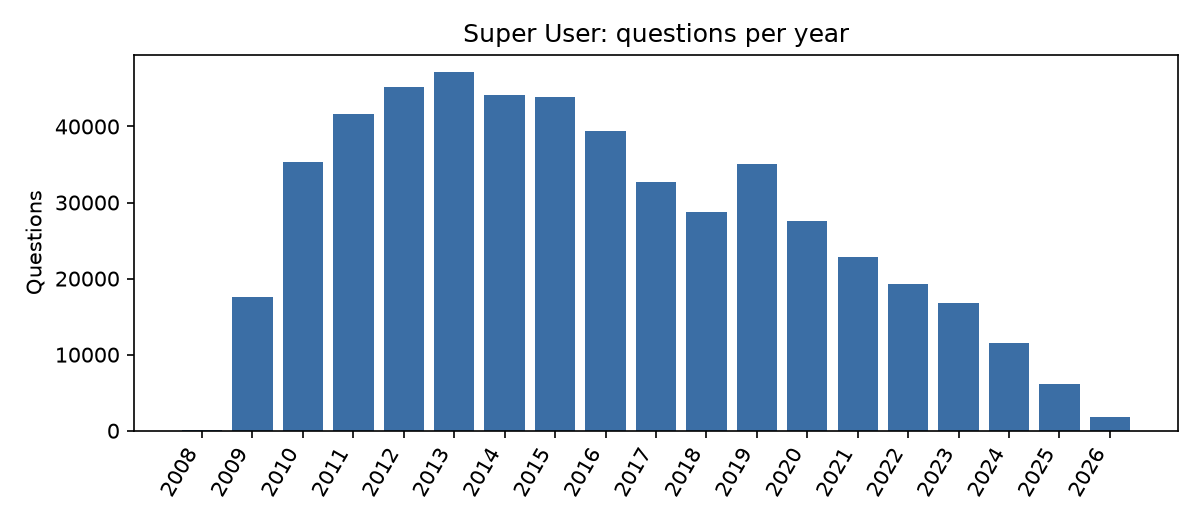
\includegraphics[height=3.0cm]{results/dataset/questions_per_year.png}\end{center}
  \vfill
  \footnotesize{\textit{Figure source: Questions per year (\texttt{results/dataset/questions\_per\_year.png})}}
\end{frame}

\begin{frame}{4. Evaluation Methodology \& Ground Truth Metrics}
  \begin{itemize}
    \item \textbf{Evaluation Metrics:}
      \begin{itemize}
        \item \textbf{Recall@K ($K \in \{1, 5, 10\}$):} per duplicate question $q$ with originals $R_q$: $|\text{top-}K \cap R_q| / |R_q|$, averaged over all such questions (macro average).
        \item \textbf{Precision@K:} $|\text{top-}K \cap R_q| / K$ (divided by $K$ even with fewer candidates), averaged the same way; a lower bound, because unlabelled duplicates count as misses.
        \item \textbf{Reduction Ratio (RR):} share of \emph{all} $N(N-1)/2$ question pairs that LSH does not have to compare:
          \[ RR = 1 - \frac{|\text{Retrieved Candidates}|}{N(N-1)/2} \]
        \item \textbf{Ranking Quality:} Mean Average Precision (MAP) and NDCG@10 for order-aware evaluation.
      \end{itemize}
    \item \textbf{Evaluation Architecture:} Single unified evaluation CLI (\texttt{src/evaluation/evaluate.py}) reading Contract C4/C5 candidates.
  \end{itemize}
  \vfill
  \footnotesize{\textit{Figure source: Metric evaluation pipeline (\texttt{src/evaluation/README.md})}}
\end{frame}

% -----------------------------------------------------------------------------
% Presenter: Iesrat Jahan (WS2)
% -----------------------------------------------------------------------------

\begin{frame}{5. Distributed Similarity Pipeline Architecture}
  \begin{itemize}
    \item \textbf{Stage Transitions:}
      \[ \text{Raw Text (C1)} \xrightarrow{\text{Shingling}} \text{Shingles (C2)} \xrightarrow{\text{MinHash}} \text{Signatures (C3)} \xrightarrow{\text{LSH}} \text{Candidates (C4)} \]
    \item \textbf{Implementation Principles:}
      \begin{itemize}
        \item 100\% custom implementation: no black-box MLlib clustering or Spark \texttt{MinHashLSH} shortcuts.
        \item Native Spark SQL and RDD \texttt{mapPartitions} arithmetic; avoids Python row-by-row UDF serialization.
        \item Memory-managed chunking (\texttt{--bands-per-pass}) to ensure execution on resource-constrained laptops.
      \end{itemize}
  \end{itemize}
  \vfill
  \footnotesize{\textit{Figure source: Pipeline contract interfaces (\texttt{docs/work\_plan.md})}}
\end{frame}

\begin{frame}[shrink=20]{6. Shingling \& Text Preprocessing (Experiment E1)}
  \begin{itemize}
    \item \textbf{HTML Sanitization:} Strips markup; word shingles keep letters, digits and \texttt{\_} and split on all other symbols.
    \item \textbf{Code Block Isolation:} Text inside \texttt{<code>} and \texttt{<pre>} is extracted into a dedicated \texttt{code\_shingles} stream.
    \item \textbf{Representation Comparison (E1):}
      \begin{itemize}
        \item Evaluated 14 options (word 1--5 grams, char 5-grams, title vs. title+body, common-shingle pruning).
        \item Highest AUC: Word 1-grams title+body with common 5\% dropped (AUC = 0.957).
        \item \textbf{Pipeline Choice:} \textbf{Word 1-grams, title only} (\texttt{word1\_title}): 35.2\% duplicate pairs reach $J \ge 0.2$; random median 0.000; only 9.6 shingles per question.
      \end{itemize}
    \item \textbf{Output:} xxHash64 values reduced modulo $2^{31}-1$ in Contract C2 (\texttt{post\_id}, \texttt{shingles}, \texttt{code\_shingles}).
  \end{itemize}
  \begin{center}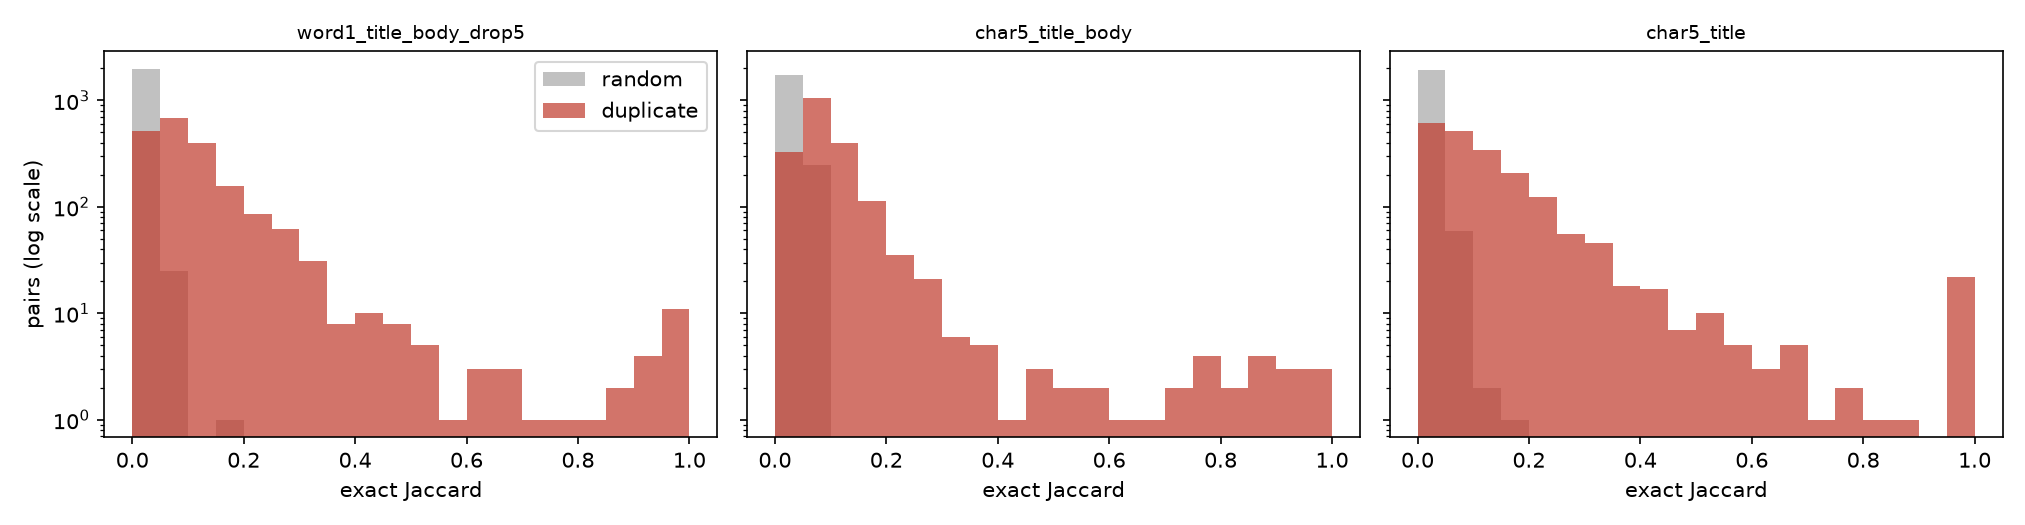
\includegraphics[height=3.0cm]{results/e1_representation/best_options_histograms.png}\end{center}
  \vfill
  \footnotesize{\textit{Figure source: Jaccard of duplicate and random pairs, best options (\texttt{results/e1\_representation/best\_options\_histograms.png})}}
\end{frame}

\begin{frame}[shrink=20]{7. MinHash Signatures from Scratch (Experiment E2)}
  \begin{itemize}
    \item \textbf{Hash Function Family:} Universal modular linear hashing:
      \[ h_i(x) = (a_i \cdot x + b_i) \bmod 2{,}147{,}483{,}647, \quad a_i, b_i \in [1, 2^{31}-2] \]
    \item \textbf{Theoretical Foundation:} $P(h_i(A) = h_i(B)) = J(A, B)$.
    \item \textbf{Signature Length Experiment (E2):}
      \begin{itemize}
        \item Tested lengths $n \in \{32, 64, 128, 256\}$.
        \item Standard error follows theoretical bound $\sigma = \sqrt{\frac{s(1-s)}{n}}$.
        \item \textbf{$n = 128$ selected:} the measured spread at $s=0.5$ is 0.049 (theory 0.044) with signatures of 1 KB per question.
      \end{itemize}
    \item \textbf{Prefix Stability:} Independent random generator guarantees shorter signatures are strict prefixes of longer ones.
  \end{itemize}
  \begin{center}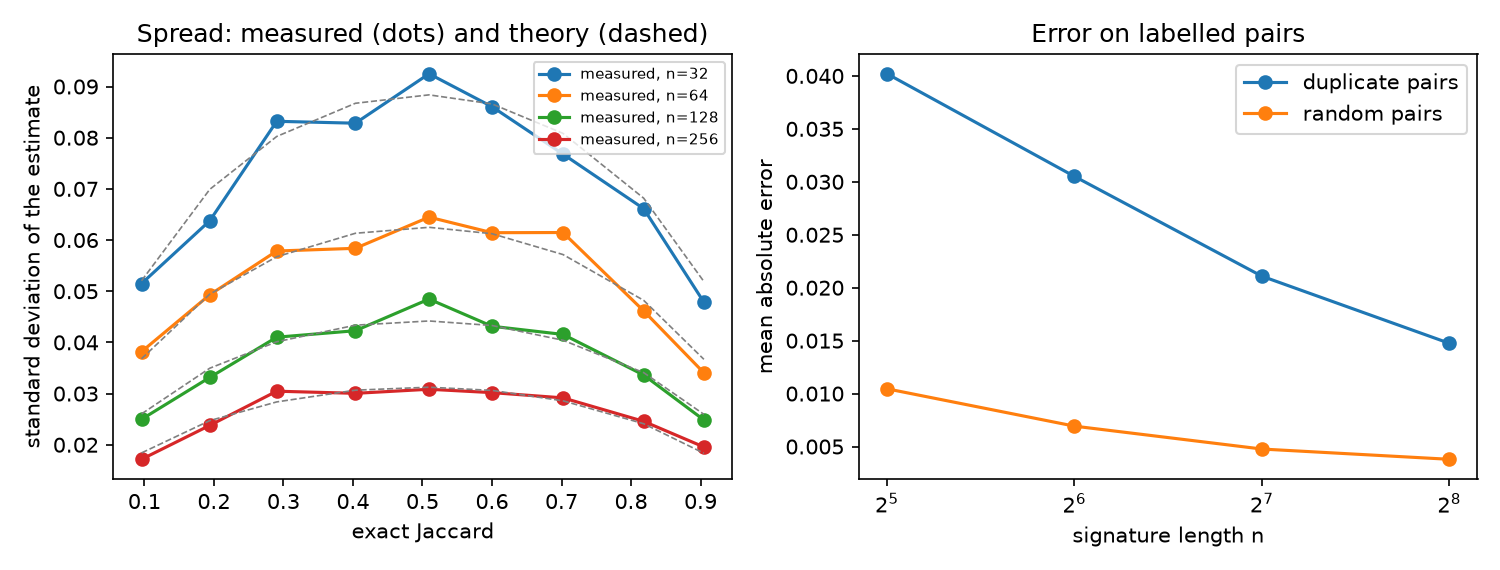
\includegraphics[height=3.0cm]{results/e2_signature/accuracy.png}\end{center}
  \vfill
  \footnotesize{\textit{Figure source: Spread of the estimate against theory (\texttt{results/e2\_signature/accuracy.png})}}
\end{frame}

\begin{frame}[shrink=20]{8. LSH Banding \& S-Curves: Theory vs. Measurement (Experiment E3)}
  \begin{itemize}
    \item \textbf{Banding Technique:} Divides $n=128$ hashes into $b$ bands of $r$ rows ($b \times r = 128$).
    \item \textbf{Theoretical Detection Probability:} $P(\text{collision} \mid s) = 1 - (1 - s^r)^b$.
    \item \textbf{Evaluated Settings (Real Super User Run on 9,583 questions):}
      \begin{itemize}
        \item \texttt{high\_precision} ($b=16, r=8$): Threshold $t \approx 0.707$, 153 candidates, Recall@10 = 1.7\%, 6\,s.
        \item \textbf{\texttt{balanced} ($b=32, r=4$):} Threshold $t \approx 0.420$, 73,889 candidates, 99.8\% reduction ratio, Recall@10 = 11.5\% (\textbf{Chosen Baseline}).
        \item \texttt{high\_recall} ($b=64, r=2$): Threshold $t \approx 0.125$, 3.89M candidates, 91.5\% reduction ratio, Recall@10 = 29.8\% (sample benchmark).
      \end{itemize}
    \item \textbf{Theory vs. Measurement:} S-curve measurements follow the predictions (mean difference 1 to 3 points per setting; up to 10 points in single bins).
  \end{itemize}
  \begin{center}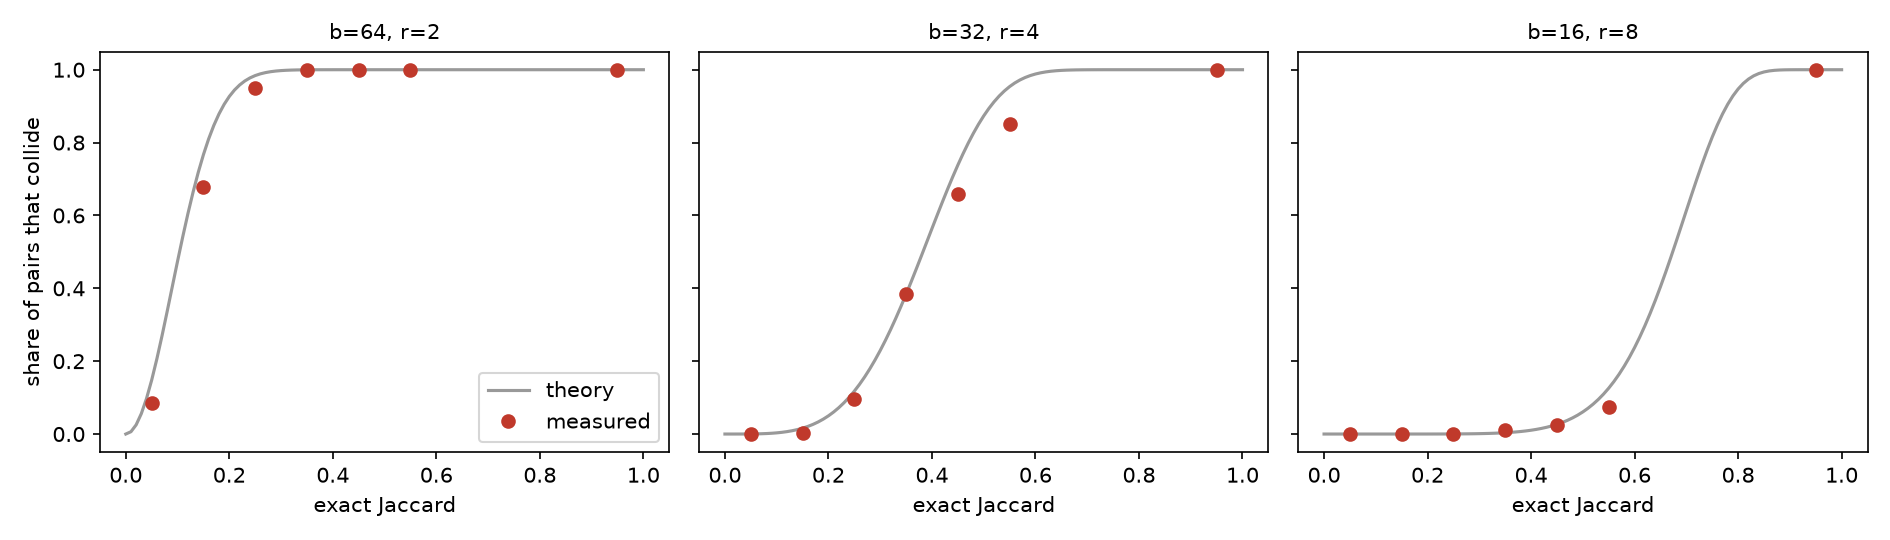
\includegraphics[height=3.0cm]{results/e3_lsh_real/s_curves.png}\end{center}
  \vfill
  \footnotesize{\textit{Figure source: S-curves: predicted vs. measured (\texttt{results/e3\_lsh\_real/s\_curves.png})}}
\end{frame}

% -----------------------------------------------------------------------------
% Presenter: Navjot Singh Shienh (WS3)
% -----------------------------------------------------------------------------

\begin{frame}{9. Big-Bucket Skew \& Pruning Policies (Experiment E7)}
  \begin{itemize}
    \item \textbf{The Skew Hazard:} a bucket of 10,000 posts implies about 50 million pairs, which one executor has to build.
    \item Without a limit, 659 of 46.4 million buckets hold \textbf{89.9\%} of all bucket pairs; the largest has 75,810 questions.
    \item \textbf{Size limit:} \texttt{size\_limit(1000)} counts each bucket's size (a shuffle), then drops buckets over 1,000 before any pair is built.
  \end{itemize}
  \begin{center}\begin{tabular}{lrrrr}
    \toprule
    Strategy & Time (s) & Candidates & Recall@10 & Slowest task (s) \\
    \midrule
    Size limit 1,000 & 3,034 & 740.0M & 3.8\% & 148 \\
    Drop common shingles (5\%) & 2,261 & 578.1M & 4.7\% & 403 \\
    \bottomrule
  \end{tabular}\end{center}
  \footnotesize{The second run had no size limit and also changed the shingles. Recall lost only to the limit is not measured.}
  \vfill
  \footnotesize{\textit{Source: \texttt{results/e7\_buckets/bucket\_profile.csv}, \texttt{bucket\_comparison.csv}}}
\end{frame}

\begin{frame}{10. Topic Partitioning \& Tag Blocking (Experiment E6)}
  \begin{itemize}
    \item \textbf{Concept:} Compare only questions in the same tag group, assuming duplicates share tags.
    \item \textbf{Blocking Mechanism (Contract Hook 2):}
      \begin{itemize}
        \item \texttt{--groups}: Maps questions to frequent tag combinations (SON algorithm itemsets) or primary tags.
        \item Group identifiers prefix bucket hash keys: items in different groups never collide in buckets.
      \end{itemize}
    \item \textbf{Empirical Impact:}
      \begin{itemize}
        \item SON groups: 60\% fewer candidates, only 8\% less time, Recall@10 down from 3.8\% to 2.7\%.
        \item Single most frequent tag: 68\% fewer candidates, 23\% less time, Recall@10 2.4\%.
        \item The assumption often fails: SON groups separate 54\% of the labelled pairs.
      \end{itemize}
  \end{itemize}
  \vfill
  \footnotesize{\textit{Source: \texttt{results/e6\_blocking/blocking\_comparison.csv}}}
\end{frame}

\begin{frame}[shrink=10]{11. Exact Verification \& Candidate Re-Ranking (Experiment E4)}
  \begin{itemize}
    \item \textbf{Refinement Pipeline (Contract C4 $\to$ C5):}
      \begin{itemize}
        \item LSH outputs candidate pairs with estimated Jaccard similarity \texttt{est\_sim}.
        \item Verification phase retrieves exact shingle sets and computes true Jaccard similarity:
          \[ J_{\text{exact}}(A, B) = \frac{|A \cap B|}{|A \cup B|} \]
      \end{itemize}
    \item \textbf{Re-Ranking Strategies Evaluated (E4):}
      \begin{itemize}
        \item \texttt{estimated}: Rank ordered by MinHash signature overlap.
        \item \texttt{exact\_jaccard}: Re-ranked by exact Jaccard similarity.
        \item \texttt{tfidf\_cosine}: Re-ranked using TF-IDF token weights (stretch).
      \end{itemize}
    \item \textbf{Results:} Exact Jaccard changes the top-1 candidate for 17.7\% of queries (top-1 agreement 82.3\%, mean rank shift 0.94). On 4,107 queries Recall@10 stays 11.5--11.6\%; Recall@1 is 8.9\% estimated, 8.7\% exact, 10.0\% TF-IDF titles, 10.5\% with bodies.
  \end{itemize}
  \vfill
  \footnotesize{\textit{Figure source: Ranking strategy comparison (\texttt{results/e4\_verification/ranking\_comparison.csv})}}
\end{frame}

% -----------------------------------------------------------------------------
% Presenter: Md Jubayer Khan (WS4)
% -----------------------------------------------------------------------------

\begin{frame}{12. Cluster Topology \& Distributed Deployment}
  \begin{itemize}
    \item \textbf{Testbed:} two 16 GB laptops joined by a wired Gigabit link.
      \begin{itemize}
        \item \textbf{Node A (Intel i7-13650HX):} HDFS NameNode and DataNode, Spark master and worker.
        \item \textbf{Node B (AMD Ryzen 7 5800H):} HDFS DataNode and Spark worker.
        \item \textbf{Full core run:} 8 cores and 8 GB on A, 4 cores and 5 GB on B, 4 GB per executor.
      \end{itemize}
    \item \textbf{Software:} Apache Spark 3.5.3 standalone, Hadoop 3.3.6 HDFS (two copies), Java 17.
    \item \textbf{Pipeline:} HDFS $\to$ shingles $\to$ MinHash $\to$ LSH $\to$ evaluation, each stage saved.
  \end{itemize}
  \vfill
  \footnotesize{\textit{Source: \texttt{results/core\_pipeline\_summary.md}}}
\end{frame}

\begin{frame}[shrink=5]{13. Baseline Comparison: Ours vs. Exact \& Spark MLlib (E5)}
  \begin{itemize}
    \item \textbf{Exact all-pairs} (two implementations, same pairs): 4.9M pairs at 10k questions, 98.8M at 50k (355 s for the faster one); 100k was not run.
    \item \textbf{One shared Super User sample} of 9,650 questions:
  \end{itemize}
  \begin{center}\begin{tabular}{lrr}
    \toprule
    Method & Candidates & Recall@10 \\
    \midrule
    Exact, $J \ge 0.1$ & 3,671,388 & 35.1\% \\
    Ours, $b=64$, $r=2$ & 3,660,207 & 33.8\% \\
    Ours, $b=32$, $r=4$ & 78,091 & 11.6\% \\
    Spark \texttt{MinHashLSH}, 5 tables, $J \ge 0.6$ & 99 & 2.4\% \\
    \bottomrule
  \end{tabular}\end{center}
  \footnotesize{Spark's 0.6 cutoff explains most of its low recall. Not compared: equal recall, or run times (two runs differed by up to 4.6 times).}
  \vfill
  \footnotesize{\textit{Source: \texttt{results/e5\_baselines/runs.csv}, \texttt{shared\_sample.csv}}}
\end{frame}

\begin{frame}[shrink=10]{14. Scalability: Cores, Machines and Data (Experiment E8)}
  \begin{itemize}
    \item \textbf{More cores} (25\%, one laptop, local files): speedup 1.69, 2.92, 3.47 on 2, 4, 8 cores; efficiency 84\%, 73\%, 43\%.
    \item \textbf{Limits:} three stages take 88--92\% of the time; median task 1.54 s $\to$ 2.44 s; longest task is 19\% of the 8-core run; Amdahl share 0.16 (rough).
    \item \textbf{Second machine} (HDFS): two laptops $\times$ 8 cores 960 s; Intel laptop alone 1,932 s; 4 to 8 cores per laptop only 1.20$\times$.
    \item \textbf{Data size: [TODO: run time against 10\%, 25\%, 50\% and 100\% of the subset, E8 test C, \#43]}
  \end{itemize}
  \begin{center}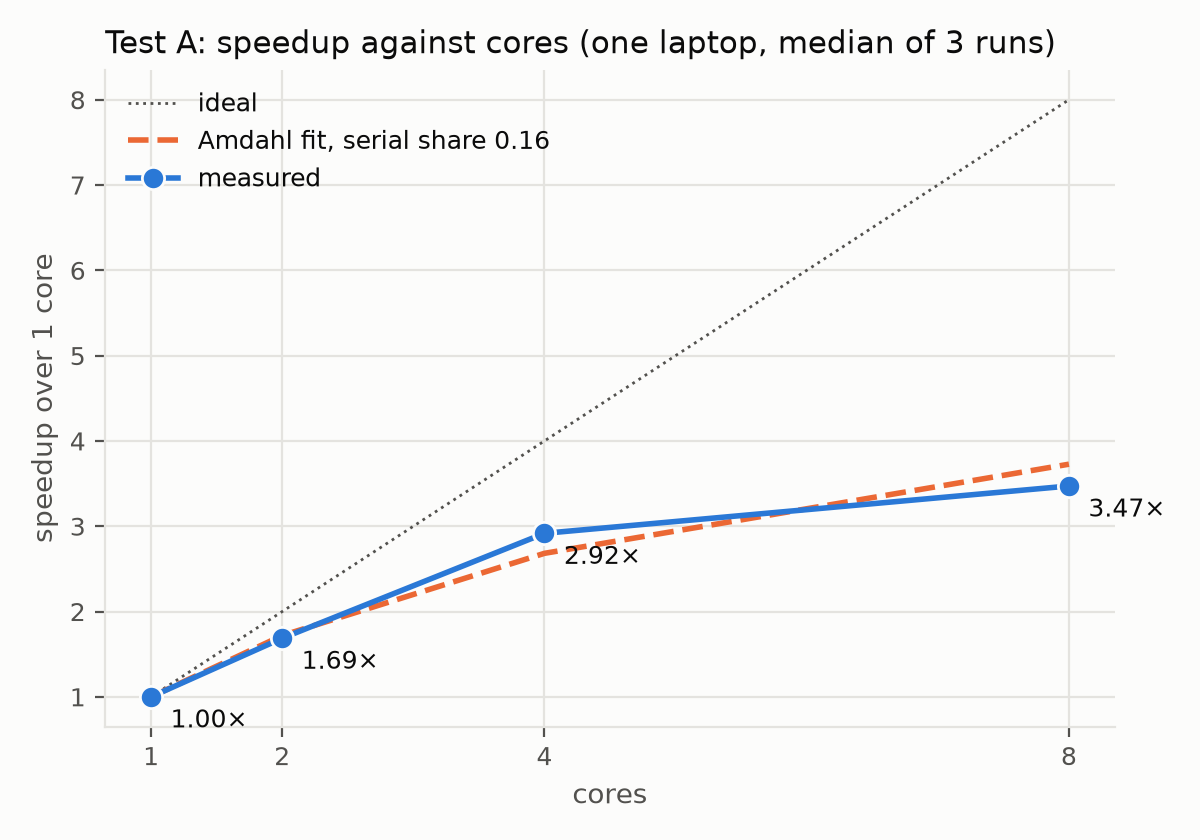
\includegraphics[height=3.2cm]{results/e8_scaling/analysis/speedup_cores.png}\end{center}
  \vfill
  \footnotesize{\textit{Source: \texttt{results/e8\_scaling/analysis/}}}
\end{frame}

\begin{frame}{15. Technical Challenges \& Engineering Solutions}
  \begin{itemize}
    \item \textbf{Challenge 1: Very large buckets}
      \begin{itemize}
        \item \textit{Answer:} \texttt{size\_limit(1000)} counts bucket sizes (one shuffle), then drops oversized buckets before pairs are built, which limits the work and memory of any one task. It does not log what it drops.
      \end{itemize}
    \item \textbf{Challenge 2: A software update during a long run}
      \begin{itemize}
        \item \textit{Answer:} an automatic update replaced Java while a job ran; we restarted the Spark services and ran that test again.
      \end{itemize}
    \item \textbf{Challenge 3: Directional Duplicate Ground Truth}
      \begin{itemize}
        \item \textit{Fix:} Each link is oriented by the \texttt{created} timestamp of its two questions (the newer is \texttt{dup\_id}), not by id order; links with equal timestamps are dropped.
      \end{itemize}
  \end{itemize}
\end{frame}

\begin{frame}{16. Summary, Impact \& Q\&A Readiness}
  \begin{itemize}
    \item \textbf{Core Results:}
      \begin{itemize}
        \item Full python subset: shingles and signatures 1,065 s; candidates and evaluation 3,571 s.
        \item Recall@10 3.8\%, reduction ratio 99.97\%; 71.3\% of labelled pairs have title similarity under 0.2.
      \end{itemize}
    \item \textbf{Course Concepts Mastered:} Locality-Sensitive Hashing, MinHash, Universal Hash Families, S-Curves, MapReduce Partitioning, RDD Optimization, Distributed Scalability.
    \item \textbf{Reproducibility:} Fully automated via frozen JSON configs and clean CLI entry points.
    \item \textbf{Ready for Defense \& Q\&A!}
  \end{itemize}
\end{frame}

\end{document}
